\documentclass[12pt]{article}

\input quiz-setup
\newcommand{\version}{} 
\newcommand{\xzero}{}
\newcommand{\xone}{}
\newcommand{\xtwo}{}
\newcommand{\xthree}{}
\newcommand{\xfour}{}
\newcommand{\xfive}{}

\newcommand{\ExamName}{Quiz \#2\version}
% \newcommand{\CourseName}{Math 34A}
% \renewcommand{\Quarter}{Spring 2017}



\begin{document}
%%
%% Version A:
\renewcommand{\version}{}
\renewcommand{\xzero}{0.0}
\renewcommand{\xone}{1.3}
\renewcommand{\xtwo}{2.9}
\renewcommand{\xthree}{4.1}
\renewcommand{\xfour}{5.3}
\renewcommand{\xfive}{6.5}
% 
\begin{minipage}{0.25\linewidth}
  \CourseName\ \Quarter \\
  \ExamName \\[1em]
  \textbf{No calculators}\\[2em]
\end{minipage}
\hfill
\begin{minipage}[t]{0.4\linewidth}
  
\begin{tikzpicture}[x=26mm,y=16mm]
    \draw[thick,black] (0,0) rectangle (3,1);
    \node[\faintcolor,right] at (0,0.2) {\large\textsf{PRINT NAME}};
  \end{tikzpicture}
\end{minipage}
\hfill
\begin{minipage}{0.25\linewidth}
  \vspace*{-3.25em}
  \ \hfill
  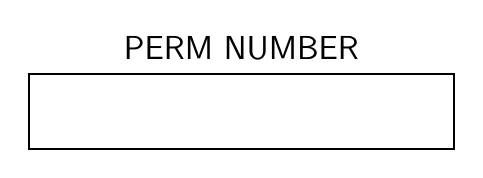
\begin{tikzpicture}[x=36mm,y=16mm]
    \node[\faintcolor] at (0.75,0.8) {\large\textsf{PERM NUMBER}};
    \draw[thick,black] (0,0) rectangle (1.5,0.6);
  \end{tikzpicture}
\end{minipage}
% \medskip
\vspace*{-0.25in}

Put your answer in the 
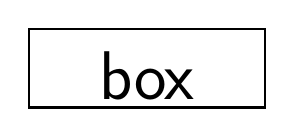
\begin{tikzpicture}[x=10mm,y=10mm,baseline=3mm] 
  \draw[thick,black] (0,0) rectangle (3,1);
  \node[\faintcolor] at (1.5,0.4) {\Huge\textsf{box}};
\end{tikzpicture}
provided.
\hfill
\begin{minipage}{0.5\linewidth}
\begin{center}

  \textbf{TA:}\ 
  \parbox[t]{0.7in}{%
    \checkbox\ \TAOne \\
    \checkbox\ \TATwo 
  }
  %\parbox[t]{0.7in}{%
  %  \checkbox\ \TAThree\\
  %  \ \ \ 
  %}
  % \ 
  % \parbox[t]{4in}{%
  % \textbf{Section Time:}
  \hfill%\hspace*{0.25in}
  % \ 
  % \parbox[t]{4in}{%
  % \textbf{Section Time:}
  \textbf{Time:}
  \parbox[t]{0.55in}{%
    \checkbox\ 4:30 \\
    \checkbox\ 5:30
  }
  \quad
  \parbox[t]{0.55in}{%
    \checkbox\ 6:30 \\
    \checkbox\ 7:30 
  }
  % }
%  \textbf{TA:}\ 
%  \parbox[t]{0.95in}{%
%    \checkbox\ \TAOne
%  }
%  \parbox[t]{0.95in}{%
%    \checkbox\ \TATwo\\
%  }
%%  \parbox[t]{0.95in}{%
%%    \checkbox\ \TAThree
%%  }
%  \hspace*{0.5in} 
%  \parbox[t]{3in}{%
%    \textbf{Section Time:}
%    \parbox[t]{0.75in}{%
%      \checkbox\ 4:30 \\
%      \checkbox\ 5:30
%    }
%    \parbox[t]{0.75in}{%
%      \checkbox\ 6:30 \\
%      \checkbox\ 7:30
%    }
%  }
\end{center}

\end{minipage}
\noindent\hspace*{-2em}\rule{\textwidth+4em}{1pt}%

\mbox{}

\begin{enumerate}
  \setcounter{problemnumber}{0}
	\Problem What is the keyword? \answerbox{6}
\end{enumerate}

\textbf{Today we will be working in groups of 3.} Discuss the following questions about exact equations with your group, and write down the answers your group comes up with. You can each write the same things, but \textbf{everyone in the group must turn in their own quiz.}

\begin{enumerate}
  \setcounter{problemnumber}{1}
	\Problem Why do you think exact differential equations are called ``exact"? {\small [There is a ``right" answer here.]} \textbf{Use complete sentences.}
	
	\vfill

  \Problem When you are deciding how to solve a given DE, what would give you the suspicion that it might be exact? {\small [Is there a form they usually come in?] }  \textbf{Use complete sentences.}
  
  \vfill
  
  \Problem If you suspect that a differential equation is probably exact, how can you know for sure?  \textbf{Use complete sentences.}
  
  \vfill
  
  \Problem How do you solve an exact differential equation?  \textbf{Use complete sentences.}
  
  \vfill
  
  \pagebreak
  \Problem Make up your own exact differential equation and solve it below. {\small [Your answer here should be different from the other members of your group] } 

	Your equation: \answerbox{8}  
	
	Solve your equation in the space below. 
	\begin{flushright}
	\answerbox{6} $= C$
	\end{flushright}
  \vfill
  \vfill
  \vfill
  \vfill
  
  \Problem Each member in turn, explain your solution to the rest of the  group. While you are listening, write each differential equation and its solution below. {\small [You don't need to copy all the work to solve, just listen to your groupmates' explanations.] } 
   	\begin{itemize}
   	\item Group member's name: \answerbox{8}
   	
   		Equation: \answerbox{7} \hfill Solution: \answerbox{7}
   	
			This groupmate presented how to solve their equation: \checkbox
			\hfill This groupmate did \textbf{not} present: \checkbox
   		\bigskip
   	
   	\item Group member's name: \answerbox{8}
   	
   		Equation: \answerbox{7} \hfill Solution: \answerbox{7}
   	
			This groupmate presented how to solve their equation: \checkbox
			\hfill This groupmate did \textbf{not} present: \checkbox
   		\bigskip
   	   	
   	\end{itemize}
  
%	\Problem \textbf{[Optional]} Here's where the optional problem goes. 
	
%	\vfill
\end{enumerate}


%\newpage
%%%
%%% Version B:
%\renewcommand{\version}{b}
%\renewcommand{\xzero}{0.0}
%\renewcommand{\xone}{1.4}
%\renewcommand{\xtwo}{3.6}
%\renewcommand{\xthree}{5.0}
%\renewcommand{\xfour}{6.1}
%\renewcommand{\xfive}{7.5}
%\setcounter{problemnumber}{0}
%% 
%\begin{minipage}{0.25\linewidth}
%  \CourseName\ \Quarter \\
%  \ExamName \\[1em]
%  \textbf{No calculators}\\[2em]
%\end{minipage}
%\hfill
%\begin{minipage}[t]{0.4\linewidth}
%  \begin{tikzpicture}[x=26mm,y=16mm]
%    \draw[thick,black] (0,0) rectangle (3,1);
%    \node[\faintcolor,right] at (0,0.2) {\large\textsf{PRINT NAME}};
%    % \node[\faintcolor] at (1.5,0.4) {\Huge\textsf{PRINT NAME}};
%  \end{tikzpicture}
%\end{minipage}
%\hfill
%\begin{minipage}{0.25\linewidth}
%  \vspace*{-3.25em}
%  \ \hfill
%  \begin{tikzpicture}[x=36mm,y=16mm]
%    \node[\faintcolor] at (0.75,0.8) {\large\textsf{PERM NUMBER}};
%    \draw[thick,black] (0,0) rectangle (1.5,0.6);
%  \end{tikzpicture}
%\end{minipage}
%% \medskip
%\vspace*{-0.45in}
%
%\begin{minipage}{0.45\linewidth}
%  Put your answer in the 
%  \begin{tikzpicture}[x=10mm,y=10mm,baseline=3mm] 
%    \draw[thick,black] (0,0) rectangle (3,1);
%    \node[\faintcolor] at (1.5,0.4) {\Huge\textsf{box}};
%  \end{tikzpicture}
%  provided.
%\end{minipage}
%\hfill
%\begin{minipage}{0.5\linewidth}
%\begin{center}

  \textbf{TA:}\ 
  \parbox[t]{0.7in}{%
    \checkbox\ \TAOne \\
    \checkbox\ \TATwo 
  }
  %\parbox[t]{0.7in}{%
  %  \checkbox\ \TAThree\\
  %  \ \ \ 
  %}
  % \ 
  % \parbox[t]{4in}{%
  % \textbf{Section Time:}
  \hfill%\hspace*{0.25in}
  % \ 
  % \parbox[t]{4in}{%
  % \textbf{Section Time:}
  \textbf{Time:}
  \parbox[t]{0.55in}{%
    \checkbox\ 4:30 \\
    \checkbox\ 5:30
  }
  \quad
  \parbox[t]{0.55in}{%
    \checkbox\ 6:30 \\
    \checkbox\ 7:30 
  }
  % }
%  \textbf{TA:}\ 
%  \parbox[t]{0.95in}{%
%    \checkbox\ \TAOne
%  }
%  \parbox[t]{0.95in}{%
%    \checkbox\ \TATwo\\
%  }
%%  \parbox[t]{0.95in}{%
%%    \checkbox\ \TAThree
%%  }
%  \hspace*{0.5in} 
%  \parbox[t]{3in}{%
%    \textbf{Section Time:}
%    \parbox[t]{0.75in}{%
%      \checkbox\ 4:30 \\
%      \checkbox\ 5:30
%    }
%    \parbox[t]{0.75in}{%
%      \checkbox\ 6:30 \\
%      \checkbox\ 7:30
%    }
%  }
\end{center}

%\end{minipage}
%\noindent\hspace*{-2em}\rule{\textwidth+4em}{1pt}%
%
%\begin{enumerate}
%  \setcounter{problemnumber}{0}
%  \Problem 
%  In your own words, what does it mean for a differential equation to be linear?
%  
%  \vfill
%  
%  \Problem Suppose you have a linear ordinary differential equation of order 2 given by $$a(t)y''+b(t)y'+d(t)y=$$ and you also have two functions $y_1$ and $y_2$ that are solutions to the differential equation. Show that $C_1y_1+C_2y_2$ is also a solution ($C_1$ and $C_2$ are constants). 
%  
%  \vfill
%  \vfill
%
%
%\end{enumerate}



\end{document}
